% Chapter 3

\chapter{A Hidden Markov Deterioration Model with Measurement Errors} % Write in your own chapter title
\label{Chapter4}
\lhead{Chapter 4. \emph{A Hidden Markov Deterioration Model with Measurement Errors}} % Write in your own chapter title to set the page header

\section{General introduction}
\label{41}
%The Markov chain model has been widely documented as an important methodology in hazard analysis of infrastructure asset management \cite{madanat95,shin,shahin05}. A good example of its application can be referred to PONTIS program, which was developed for bridge management \cite{pontis}. Fundamentally, Markov chain model is applied for forecasting the deterioration process, performance of infrastructure over time. In the model, discrete states are classified to represent the performance condition of infrastructure. The deterioration, as transition pattern among states, is simulated as stochastic process based on theory of Markov chain. 
%
Application of Markov hazard models requires monitoring data from at least two inspection times. Thus, the accuracy of estimation largely depends on the quality of monitoring data. Errors exist in monitoring data are referred as measurement errors arising from measurement system or inspector (human or machine), inspected objects, or from data processing and data interpretation \cite{humplick}. Measurement errors tend to cause  estimation results to be different from what they should be, especially under a small pool of monitoring data.

This chapter proposes a hidden Markov deterioration model, with an innovative analytical method to eliminate the negative influence of measurement errors on estimation results. In the model, measurement errors are assumed as random variables. In addition, the functional relation between the ``true condition states'' and ``measurement errors'' of an infrastructure component is formulated by a mixture mechanism. Precisely, the mixing mechanism is referred as the dispersion of the ``observed condition states'' to the ``true condition states''. To estimate the parameters of the model, we apply the method of maximum likelihood, together with the  Bayesian estimation and MCMC simulation.

The following section presents a framework on measurement errors and the process of deterioration with hidden condition states. Section \ref{44} details the mathematical formulation of mixture distribution and hidden Markov transition probability. An analytical technique using Bayesian estimation and MCMC simulation is discussed in section \ref{45}. Section \ref{46} illustrates an empirical study using data of Japanese national road system. The last section summarizes contributions of the model and further includes a discussion for future research.
%%%%%%%%%%%%%%%%%%%%%%%%%%
\section{Measurement errors and hidden condition states}
\label{42}
\subsection{Measurement errors and the problem of representative values}
\label{421}
In infrastructure management practices, the healthy status or performance of an infrastructure component is described in discrete condition states, which are defined by means of a single performance index or an aggregate index. The values of indexes are measured by monitoring and visual inspection. For example, in the case of pavement management system (PMS), the condition states include the extend of several pavement distress such as rut and cracking, or some aggregate condition states, such as the Pavement Condition Index (PCI) \cite{shahin05}.

However, because of measurement errors, the true condition states may not be captured. Fig. \ref{fig41} presents a problem of having measurement errors in the PMS. The values on both horizontal and vertical axes indicate the rut index, which are measured at inspection time $\tau_A$ and $\tau_B~(\tau_A<\tau_B)$ respectively. If there is no maintenance and repair ($M\&R$) actions during the past inspection period ($6$ years), the dots representing the values of ruts should be located above the $45^o$ line. However, as can be seen from the figure, a great numbers of dots are  located under the $45^o$ line, inferring measurement errors. As a result, the observed condition states representing by the dots under the $45^o$ line might be used in the hazard analysis instead of using the true condition states. The problem of representation of condition states is referred as the ``representation matter''.

%%%
\begin{figure}
\begin{center}
\begin{footnotesize}
\includegraphics[scale=0.5]{fig41.eps}\\
Note) Samples under the $45^0$ line represent the values of the rut index for road sections. \\
\caption{Measurement errors in pavement management system.}
\label{fig41}
\end{footnotesize}
\end{center}
\end{figure}
%%%%%%%
\subsection{The process of deterioration in hidden Markov hazard model} \label{422}
A clear picture of measurement errors can be seen from Fig. \ref{fig42}. In the figure, the  deterioration of a road section is described as the transition pattern among condition states $i$ $(i=1,...,I)$, with $i=1$ as the new condition state and $i=I$ as the worst condition state (absorbing condition state). Two visual inspections are supposed to be carried at inspection times $\tau_A$ and $\tau_B$. In addition, there is no $M\&R$ action during the interval $[\tau_A$, $\tau_B]$. The observed condition state of the road section at inspection times $\tau_A$ and $\tau_B$ are $m(\tau_A)=m(m=1,...,I)$ and $n(\tau_A)=n(n=1,...,I) (m \leq n)$ respectively. However, because of measurement errors, the observed condition state is different from the true condition state, which is supposed to be equal to  $m^\ast(\tau_A)=i~(i=1,\cdots,I)$ at times $\tau_A$ and $m^\ast(\tau_B)=j~(j=1,\cdots,I)$ at times $\tau_B$.

In monitoring practices, to quantify the condition state of a road section, several values of distress are examined. However, inspectors tend to select the worst condition state  among the observed condition states of distress to be the representative condition state of that section. As can be seen from the Fig. \ref{fig42}, the ``true condition state'' $m^\ast(\tau_A)=i$ at times $\tau_A$ is lower than the ``observed condition state'' $m(\tau_A)=m$ at times $\tau_B$. 

\begin{figure}
\begin{center}
\begin{footnotesize}
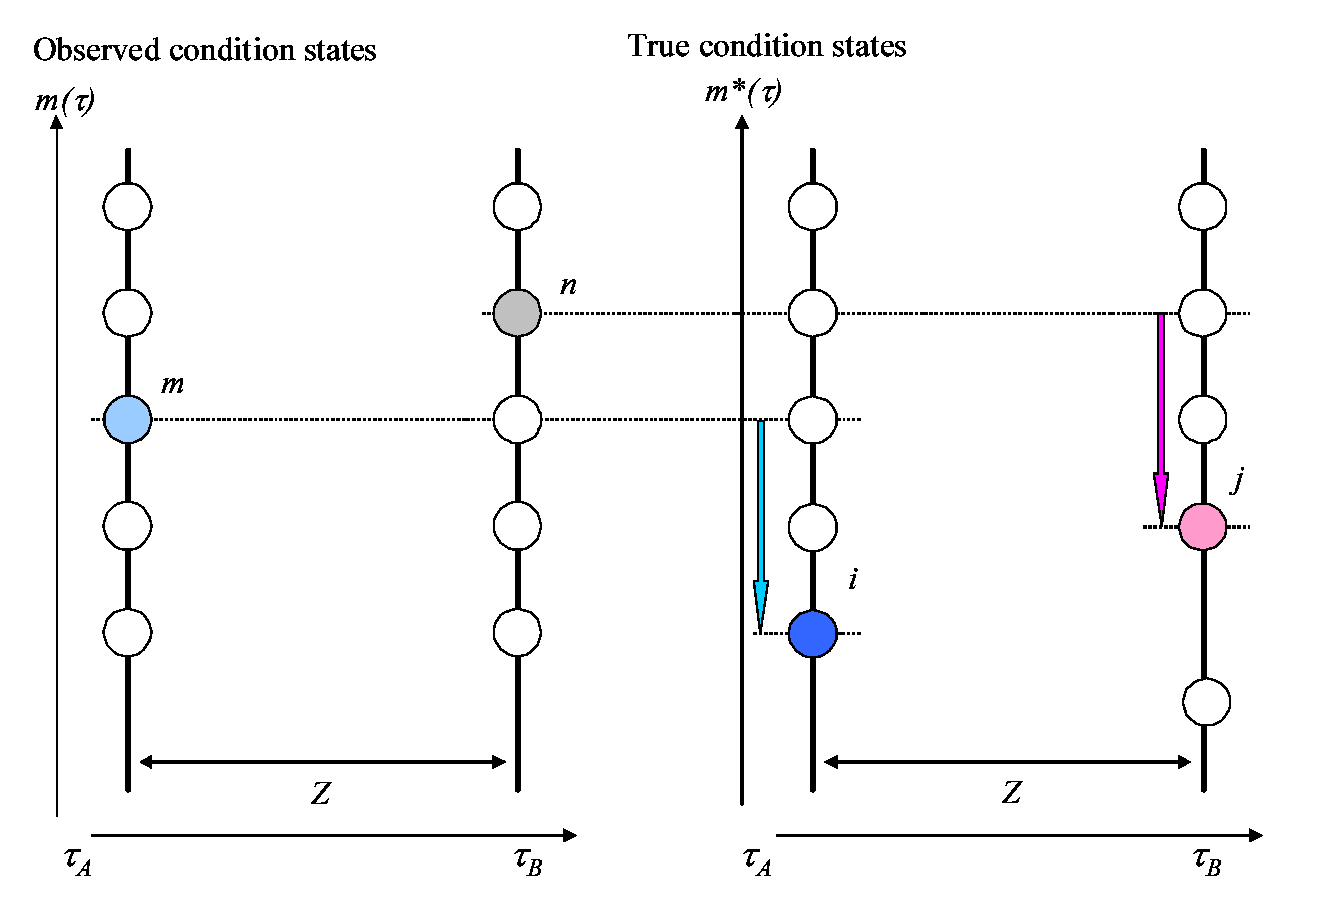
\includegraphics[scale=0.5]{fig42.eps}\\
Note) Observed values of states for $\tau_A, \tau_B$ are higher than the true condition state values due to measurement errors.
\end{footnotesize}
\end{center}
\caption{Degree of Measurement Errors.}
\label{fig42}
\end{figure}
%%%

According to \citet{humplick}, measurement errors can be assigned as random variables. With this assumption, the discrete probability distribution of observed condition state $m$ can be described by using likelihood function $f_i(m|\mbox{\boldmath$\alpha$}_i)$. We can explain from the function that the probability of the observed condition state $m$ conditionally depends on the true condition state $i$. In other words, it conditionally depends on the characteristic parameter $\mbox{\boldmath$\alpha$}_i$ of the probability distribution of the true condition state $i$.

We further assume $z$ as the duration between two consecutive inspection times $\tau_A$ and $\tau_B$. On the same road section, at inspection time $\tau_B$, the observed condition states and true condition states are supposed to be $m(\tau_B)=n$ and $m^\ast(\tau_B)=j$ respectively. Since the process of deterioration progresses in an  uncertain manner, there is no concrete guarantee of having any correlation between the two  condition states $n$ and $j$. 

As for the transition pattern between the condition states in the period $[\tau_A,\tau_B)$, it is $m\rightarrow n$ for the observed condition states and $i\rightarrow j$ for the true condition states. In term of Markov transition probability, however, we are able to estimate only the Markov transition probability $\pi_{mn}$, while  the Markov transition probability $\pi_{ij}$ is hidden. Because of the hidden characteristics, the hidden Markov model is then proposed, with its focus on estimating  the true Markov transition probability $\pi_{ij}$. Further to the meaning of the likelihood function $f_i(m|\mbox{\boldmath$\alpha$}_i)$, it can be described as a mixing part of the conventional Markov transition probability (refer to Chapter \ref{Chapter2}). Thus, one of important roles of the hidden Markov model is to estimate the condition probability distribution $f_i(m|\mbox{\boldmath$\alpha$}_i)$.
%%%%
\section{Exponential Markov Deterioration Hazard Model}
\label{43}
Reference is mainly made to section \ref{233}, in which, the exponential Markov Hazard model has been extensively explained. For convenience of reading in subsequent parts of this Chapter, following equation is given as  the obtained results from section \ref{233} in Chapter \ref{Chapter2}:
%
\begin{eqnarray}
&& \pi_{ij}(z)=\mbox{Prob}[m^\ast(\tau_B)=j|m^\ast(\tau_A)=i]  =\prod_{m=i,\neq k}^{k-1}\frac{\theta_m}{\theta_{m}-\theta_{k}} \exp (-\theta_{k}z). \label{4poi}
\end{eqnarray}
\section{Hidden Markov hazard model} \label{44}
\subsection{Mixture distribution mechanism} \label{441}
%
This section explains the mathematical formulation of the hidden Markov chain model based on mixture distribution mechanism. Assumption is referred to section \ref{422}. In fact, it is uncertain to use the probability distribution function $f_i(m|\mbox{\boldmath$\alpha$}_{i})~(i=1,\cdots,I)$ to estimate the true condition state $i$. However,  we are able to express the probabilistic dependence of the observed condition state $m(\tau_A)=m$ on the true condition state $i$ by means of the likelihood function $f_i(m|\mbox{\boldmath$\alpha$}_{i})~(i=1,\cdots,I)$:

\begin{eqnarray}
&& \ell(m(\tau_A)=m)=\sum_{i=1}^I \pi_i(\tau_A)
f_i(m|\mbox{\boldmath$\alpha$}_{i}).\label{mixture1}
\end{eqnarray}
where $\pi_i(\tau_A)$ is the probability of the true condition state $i$ at inspection time $\tau_A$. Equation (\ref{mixture1}) depicts the conditional probability distribution of the observed condition state $m(\tau_A)=m$ on the true condition state $i$. In other words, it portrays the conditional probability distribution of the observed condition state $m(\tau_A)=m$ by averaging the distributed values of measurement errors over the range of the true condition states. A model with mixing mechanism of measurement errors is referred as a mixture distribution model \cite{die}.

Similarly, the probability distribution of the observed condition states at inspection time $\tau_B=\tau_A+z$ $(\tau_A<\tau_B)$ can be described by means of mixing form. The likelihood function $\ell(m(\tau_A)=m,m(\tau_B)=n)$, to which the observed condition state $m(\tau_B)=n$ at inspection time $\tau_B$ can be defined as
\begin{eqnarray}
&& \ell_i(m(\tau_B)=n)=\sum_{j=i}^I \pi_{ij}(z) f_j(n|\mbox{\boldmath$\alpha$}_j).
\end{eqnarray}
As a matter of course, the likelihood distribution function of the observed condition state $\ell(m(\tau_B)=n)$ at inspection time $\tau_B$ conditionally depends on the probability $\pi_i(\tau_A)$ despise the fact that the true condition state $i$ at inspection time $\tau_A$ is absolutely hidden. Following equation details the conditional dependency in the likelihood function:
\begin{eqnarray}
&& \hspace{-10mm}\ell(m(\tau_B)=n) =\sum_{i=i}^I \pi_i(\tau_A) \ell_i(m(\tau_B)=n) = \sum_{i=i}^I \pi_i(\tau_A) \sum_{j=i}^I \pi_{ij}(z) f_j(n|\mbox{\boldmath$\alpha$}_j). \label{ku}
\end{eqnarray}
As a result, the likelihood function $\ell(m(\tau_A)=m,m(\tau_B)=n)$, at which we observe the condition state $m(\tau_A)=m$ at inspection time $\tau_A$ and the condition state $m(\tau_B)=n$ at inspection time $\tau_B$, can be defined:
\begin{eqnarray}
&& \hspace{-10mm} \ell(m(\tau_A)=m,m(\tau_B)=n) = \sum_{i=1}^I \pi_i(\tau_A) f_i(m|\mbox{\boldmath$\alpha$}_{i})\left(\sum_{j=i}^I \pi_{ij}(z)  f_j(n|\mbox{\boldmath$\alpha$}_j)\right). \label{ksu}
\end{eqnarray}
It is noticed from equation (\ref{ksu}) that the probability distribution functions $f_i(m|\mbox{\boldmath$\alpha$}_{i})$ and $f_j(n|\mbox{\boldmath$\alpha$}_{j})$ are in strong correlation with each others through the Markovian transition probability $\pi_{ij}(z)$. In other words, the distribution of the observed condition state depends on the hidden characteristics or measurement errors at respective inspection time $\tau_A$ and $\tau_B$.
%%%%%%%%%%%%
\subsection{Initial values of the condition states} \label{442}
As can be seen from equation (\ref{ksu}), there are three unknown components, the initial distribution $\pi_i(\tau_A)$, the probability distribution function $f_i(m|\mbox{\boldmath$\alpha$}_{i})$ and the Markov transition probability $\pi_{ij}(z)$. The value of the initial probability distribution $\pi_i(\tau_A)$ is regarded as a transcendental information. The initial probability distribution can be assumed as a variable of non-parametric distribution. However, assuming it as a non-parametric variable limits the study for a large number of monitoring data since characteristic variables  concerning a road section do not share the same values with the other road sections. It is therefore advisable to determine the initial value of condition state immediately after any $M\&R$ action. Because, by implementing $M\&R$ actions, the condition state of a road section will become good again, with $i=1$. For example, if a $M\&R$ action is carried out just before time $\tau_0$, the initial probability distribution can be defined as
\begin{eqnarray}
&& \mbox{\boldmath$\pi$}(\tau_0)=\{\pi_1(\tau_0),\cdots,\pi_I(\tau_0)\} =(1,0,\cdots,0).
\end{eqnarray}
Evidently, the properties of the vector $\mbox{\boldmath$\pi$}(\tau_0)$ is measurable. Thus, if $M\&R$ actions are implemented at alternative times $\tau_1,\cdots,\tau_T$, the initial value of probability distribution $\pi_i(\tau_A)$ can also be defined. To come up with a general likelihood function for the conditional probability distribution of the observed condition states $m$, the observed condition states after $M\&R$ actions at times $\tau_t$ $(t=1,...,T)$ are assumed as $m(\tau_t)=m_t$. The durations between two consective $M\&R$ actions from $t-1$ to $t$ are denoted as $z_{t}~(t=1,\cdots,T)$. As a result, likelihood function ${\cal L}(\mbox{\boldmath$\alpha$},\mbox{\boldmath$m$},\mbox{\boldmath$z$})$, which describes the conditional probability distribution of the observed condition states $\mbox{\boldmath$m$}=(m_1,\cdots,m_T)$, can be recurrently defined:
\begin{eqnarray}
&& {\cal L}(\mbox{\boldmath$\alpha$},\mbox{\boldmath$m$},\mbox{\boldmath$z$})=\sum_{j=1}^I \pi_{1j}(z_1)f_j(m_1|\mbox{\boldmath$\alpha$}_j)\ell_j(1), \label{mu0} \\
&& \ell_h(t)=\sum_{j=h}^I \pi_{hj}(z_t)f_j(m_t|\mbox{\boldmath$\alpha$}_j)\ell_j(t+1) \hspace{10mm}(1 \leq t \leq T-1), \\
&& \ell_h(T)=\sum_{j=h}^I \pi_{hj}(z_T)f_j(m_T|\mbox{\boldmath$\alpha$}_j). \label{myuudo1}
\end{eqnarray}
The maximum likelihood estimation method can be used to estimate the parameters of the model by applying numerial analysis with the objective likelihood function. However, the method exerts to have its limitation as it requires a high order of derivative and high degree of computation for solving the optimal condition of nonlinear polynomial equations.  Therefore, in view of problems in the hidden Markov model, the maximum likelihood method is not deemed as an ultimate solution \cite{titter}. Attempts to overcome the limitation of the maximum likelihood method by using Bayesian estimation have been proposed.  
%%%%%%%%%%%%%%%%%%
\subsection{Complete likelihood function} \label{443}
The distribution of measurement errors is assumed by means of a hidden variable $\mbox{\boldmath$s$}=(s_0,\cdots,s_T)$. If there is no $M\&R$ action in the inspection period, the  following condition is satisfied:
\begin{eqnarray}
&& s_0=1\leq s_1 \leq \cdots \leq s_T \leq I. \label{stk}
\end{eqnarray}
Furthermore, if the hidden variable is measureable, its value can be used to update the probability distribution of the true condition state $i$, which is hidden because of measurement errors. In addition, to identify the possibility of actual measurement of the hidden variable, a dummy variable $\delta$ is assigned with the conditions as follows:
\begin{eqnarray}
&& \delta_{ti}=\left\{
\begin{array}{ll}
1 & s_t=i\\
0 & s_t\ne i
\end{array},
\right. (t=1,\cdots,T;i=1,\cdots,I) .
\end{eqnarray}
With this assumption and according to \citet{demp}, the likelihood functions (\ref{mu0})-(\ref{myuudo1}) are then  described as follows:
\begin{eqnarray}
&& \hspace{-10mm}\tilde{\cal L}(\mbox{\boldmath$s$},\mbox{\boldmath$\alpha$},\mbox{\boldmath$m$},\mbox{\boldmath$z$}) =\prod_{i=1}^I \Big\{\pi_{1i}(z_1)^{\delta_{1i}} f_{i}(m_1|\mbox{\boldmath$\alpha$}_{i})^{\delta_{1i}}  \prod_{t=2}^T \prod_{j=i}^I \pi_{ij}(z_t)^{\delta_{t-1i}\delta_{tj}} f_{j}(m_t|\mbox{\boldmath$\alpha$}_{j})^{\delta_{tj}}\Big\} \nonumber \\
&& \hspace{10mm}=\prod_{t=1}^T \Big\{\pi_{s_{t-1}s_t}(z_t) f_{s_t}(m_t|\mbox{\boldmath$\alpha$}_{s_t})\Big\} = \prod_{t=1}^T \pi_{s_{t-1}s_t}(z_t) \prod_{t=1}^T f_{s_t}(m_t|\mbox{\boldmath$\alpha$}_{s_t}). \label{hyuudo2}
\end{eqnarray}
Equation (\ref{hyuudo2}) is referred as a complete likelihood equation \citep{dani-hed}, with a better explicit form than that in the likelihood equations (\ref{mu0})-(\ref{myuudo1}). Nevertheless, a difficulty remains at this point is how to assign a realistic value for the hidden variable $\mbox{\boldmath$s$}$ since it is unobservable. In view of probability distribution, the hidden variable $\mbox{\boldmath$s$}$ can be derived by applying the full conditional posterior distribution in Bayesian inference. In which, the prior probability distribution in Bayesian estimation is assumed as follows: 
%%%%%%%%
\begin{eqnarray}
&& \hspace{-15mm} \mbox{Prob}\{s_t=i|\mbox{\boldmath$s$}_{-t},\mbox{\boldmath$\alpha$},\mbox{\boldmath$\xi$}\} =\frac{\tilde{\cal L}(\mbox{\boldmath$s$}_{-t}^i,\mbox{\boldmath$\alpha$},\mbox{\boldmath$m$},\mbox{\boldmath$z$})}{\sum_{i=s_{t-1}}^{s_{t+1}} \tilde{\cal L}(\mbox{\boldmath$s$}_{-t}^i,\mbox{\boldmath$\alpha$},\mbox{\boldmath$m$},\mbox{\boldmath$z$})} =\frac{\omega_{it} f_i(m_t|\mbox{\boldmath$\alpha$}_i)}{\sum_{j=s_{t-1}}^{s_{t+1}} \omega_{jt} f_j(m_t|\mbox{\boldmath$\alpha$}_j)}, \label{hhu}
\end{eqnarray}
where $\mbox{\boldmath$s$}_{-t}=(s_1,\cdots,s_{t-1},s_{t+1},\cdots,s_{T}),\mbox{\boldmath$s$}_{-t}^i=(s_1,$$\cdots,$$s_{t-1},i,s_{t+1},\cdots,s_{T})$, and $s_t=i ~(i$ $\in \{s_{t-1},$$\cdots, s_{t+1}\})$. In addition, $\omega_{jt}$ satisfies 
\begin{eqnarray}
&& \omega_{jt}=\left\{
\begin{array}{ll}
\pi_{1j}\pi_{js_2} & t=1 \\
\pi_{s_{t-1}j}\pi_{js_{t+1}} & 2\leq t \leq T \\
\pi_{s_{T-1}j} & t=T
\end{array}.
\right.
\end{eqnarray}
It is clear at this point that if the posterior probability distribution of the hidden variable $s_t \in \{s_{t-1},\cdots,s_{t+1}\}$ at time $t$ is measurable, the transition probability $\pi_{ij}(z)~(i=1,\cdots,I;j=i,\cdots,I)$ and the probability distribution function $f_i(m|\mbox{\boldmath$\alpha$}_i)~(i=1,\cdots,I)$ can be ultimately estimated. It is also noted that the posterior probability distribution of the hidden variable $s_t \in \{s_{t-1},\cdots,s_{t+1}\}$ is conditionally depended on the observed value of $\mbox{\boldmath$s$}_{-t}$. 

To solve the likelihood equation (\ref{hyuudo2}), it is required to estimate the value of  hidden variable $\mbox{\boldmath$s$}$. As a result, the main task is to estimate the unknown parameters $\mbox{\boldmath$\alpha$}$ and $\mbox{\boldmath$\beta$}$, which are embedded in the transition probability functions. In fact, there is no possibility to seek for the posterior distribution of all hidden variables. Thus, MCMC simulation is recommended to use in randomly generating the hidden variable $\mbox{\boldmath$s$}$.
%%%%%%
\subsection{Conditional distribution of measurement errors} \label{444}
As earlier mentioned in section \ref{42}, the representative condition state of a road section generally happens to be the worst condition state among several condition states observed on the same section. Thus, it is possible to assume the range of observed condition state $m$ in a domain $m(m=1,...,i)$. The relationship between the observed condition state $m$ and the true condition state $i$ implies measurement errors on the same road section. Suffice it to say that the selection of the observed condition state can be considered as a random selection process. However, probabilistic inference on the value of probability distribution function $f_i(m|\mbox{\boldmath$\alpha$}_i)~(m=1,\cdots,i)$ faces some degrees of difficulty. In this research, the distribution probability function $f_i(m|\mbox{\boldmath$\alpha$}_i)~(m=1,\cdots,i)$ is assigned to satisfy the following conditions:
%%%%
\begin{eqnarray}
&& f_i(m|\mbox{\boldmath$\alpha$}_i)=\left\{
\begin{array}{ll}
0 &  \hspace{10mm} when \hspace{10mm}m > i \\
\alpha_{m}^i & \hspace{10mm} when \hspace{10mm}m \leq i
\end{array},
\right. \label{pmi}
\end{eqnarray}
where parameter $\alpha_{m}^i$ is assumed as a non-parametric constant satisfying
\begin{eqnarray}
0\leq \alpha_{m}^i \leq 1, \label{a14} \\
\sum_{m=1}^i \alpha_{m}^i=1. \label{a24}
\end{eqnarray}
The probability distribution of parameter $\alpha_m^i$ can be estimated if having enough numbers of monitoring data. This is a non-parametric approach in case of receiving no prior information regarding measurement errors. This approach has been applied in the research on the probabilistic measurement of system errors \cite{bauer,jj}. 
%%%%
\section{Estimation methodology} \label{45}
\subsection{Markov Chain Monte Carlo method} \label{451}
In statistic with Bayesian inference, the prior and posterior probability are employed with aim to estimate the values of model's parameters \cite{wago}. However, in hazard analysis, it is hard to define the prior probability distribution, even in a simple condition states hazard model \cite{ibra1}. Methods to overcome the problems in the assumption of the prior probability distribution often require numerical analyses with multi-dimensional integration, and thus remain as a limitation in Bayesian estimation.

In recent years, an appealing solution to the problem in Bayesian estimation has been proposed, with the application of MCMC simulation. The MCMC simulation technique does not require a high level of derivative and multi-dimensional integration of model's objective functions \cite{wago}. As a result, estimation results in a great deal of applied statistic research have been improved through a combination of the Bayesian estimation and MCMC simulation.

In MCMC simulation, Gibbs sampling and Metropolis Hastings (Metropolis-Hastings or MH) techniques have been extensively discussed \cite{wago}. Reference to the research on image restoration is a good example of MCMC simulation \cite{gibbs1}. Of that study, the algorithm of Gibbs sampling was used to estimate the posterior distribution in Bayesian estimation \cite{gibbs2}. In MH law, the iterative parameter $\mbox{\boldmath$\beta$}$ is defined by repeatedly generating random numbers through the conditional probability density function. In this research, we propose an extended estimation methodology to estimate the parameters of the hidden Markov model based on the literature of the Bayesian estimation for the Weibull hazard model of \citet{bayse}.

Further to the estimation parameters in hidden Markov models, analytical approach using the method of maximum likelihood has already exhibited its limitation \cite{titter,robert}. Since hidden Markov model is considered as one type of mixture distribution model, a great deal of research suggested to define a set of complete likelihood functions instead of using conventional likelihood functions \cite{die,robe}. In view of MCMC simulation, it is necessary to develop an explicit algorithm for estimating the Markov transition probability with multi-condition states. In this research, we propose an analytical approach using Bayesian estimation and MCMC simulation for estimating the Markov transition probability of the conventional exponential hazard model, which is briefly presented in Chapter \ref{Chapter2}.
%%%%%%%%%%%%%%%%%%%%%%%%
\subsection{Formulation of the model} \label{452}
Visual inspection is carried out on each section $k$ of the entire road system (with $K$ is the total number of road sections). The observed data on each section over a time-series can be denoted as $\tau_t^k~(t=1,\cdots,T^k)$, with $T^k$ as the number of inspection times for the road section $k$. Each observed condition state from the visual inspection is represented as $\bar{m}(\tau_t^k)$, with the sign $\bar{\hspace{2mm}}$ indicating the measurable data. $\bar{\mbox{\boldmath$\xi$}}=(\bar{\mbox{\boldmath$\xi$}}^1,\cdots,\bar{\mbox{\boldmath$\xi$}}^K)$ is denoted as the vector of measureable data concerning $\sum_{k=1}^K T^k$ numbers of records. 

The deterioration process of a road section is influenced by the changes in the values of characteristic variables such as traffic volume, thickness of overlay, weather, etc. The values of  characteristic variables are recorded and stored in monitoring data. To consider the effects of characteristic variables on the deterioration, vector $\bar{\mbox{\boldmath$x$}}_t^k$ is assumed to represent for characteristic variables. In addition, the duration between two consecutive visual inspections is defined as $\bar{z}_t^k=\tau_t^k-\tau_{t-1}^k$. In summary, the observed information concerning each section of a road can be symbolized as $\bar{\mbox{\boldmath$\xi$}}_t^k=(\bar{m}_t^k,\bar{z}_t^k,\bar{\mbox{\boldmath$x$}}_t^k)$, with $m(\tau_t^k)=\bar{m}_t^k$. As a result, the simultaneous probability distribution for the entire $K$ samples can be defined:
%%%%%%%%
\begin{eqnarray}
&& \hspace{3mm}\tilde{\cal L}(\mbox{\boldmath$\alpha$},\mbox{\mbox{\boldmath$s$},\boldmath$\beta$},\bar{\mbox{\boldmath$\xi$}}) 
=\prod_{k=1}^K\Bigl\{\prod_{t=1}^{T^k}\pi_{s_{t-1}^ks_t^k}(\bar{z}_t^k)\prod_{t=1}^{T^k} f_{s_t^k}(\bar{m}_t^k|\mbox{\boldmath$\alpha$}_{s_t^k})\Bigl\}\nonumber \\
&& =\prod_{k=1}^K \Bigl[\prod_{t=1}^{T^k}\alpha_{\bar{m}_t^k}^{s_{t}^k}\sum_{l=s_{t-1}^k}^{s_t^k}\Bigl\{ \prod_{i=s_{t-1}^k,\neq l}^{l-1}\frac{\theta_{i}^k}{\theta_{i}^k-\theta_{l}^k}\exp(-\theta_{l}^k\bar{z}_t^k)\Bigl\}\Bigl],
\label{hyuudo3}
\end{eqnarray}
In likelihood equation (\ref{hyuudo3}), the hazard function is described by using exponential form as
$\theta_i^k=\exp(\mbox{\boldmath$x$}^k\mbox{\boldmath$\beta$}_i^\prime)$. In order to estimate the unknown parameters and the hidden variables (measurement errors), the method using to solve the likelihood functions (\ref{mu0})-(\ref{myuudo1}) should be considered. By solving equation (\ref{hyuudo3}), the values of $\mbox{\boldmath$\alpha$}=(\mbox{\boldmath$\alpha$}_1,\cdots,\mbox{\boldmath$\alpha$}_{I-1})$, $\mbox{\boldmath$\beta$}=(\mbox{\boldmath$\beta$}_1,\cdots,\mbox{\boldmath$\beta$}_{I-1})$ and hidden variable $\mbox{\boldmath$s$}=(\mbox{\boldmath$s$}^1,\cdots,\mbox{\boldmath$s$}^K)$ can be obtained. If parameter vectors $\mbox{\boldmath$\alpha$}$ and  $\mbox{\boldmath$\beta$}$ are known, the posterior distribution of the hidden variable $s_t^k~(t=1,\cdots,T^k;k=1,\cdots,K)$ can be estimated as well. Given the condition $\mbox{\boldmath$s$}_{-t}^k=(s_1^k,\cdots,s_{t-1}^k,s_{t+1}^k,\cdots,s_{T^k}^k)$, the conditional probability, to which the hidden variable $s_t^k ~(s_t^k \in \{s_{t-1}^k,\cdots, s_{t+1}^k\})$ equals to the true condition state $i$ , is finally estimated:
%%%%%%%%%%%%
\begin{eqnarray}
&& \mbox{Prob}\{s_t^k=i|\mbox{\boldmath$s$}_{-t}^k,\mbox{\boldmath$\alpha$},\mbox{\boldmath$\xi$}\} =\frac{\omega_{it}^k f_i(m_t^k|\mbox{\boldmath$\alpha$}_i)}{\sum_{j=s_{t-1}^k}^{s_{t+1}^k} \omega_{jt}^k f_j(m_t^k|\mbox{\boldmath$\alpha$}_j)},\label{k3}
\end{eqnarray}
where
\begin{eqnarray}
&& \omega_{jt}^k=\left\{
\begin{array}{ll}
\pi_{1j}\pi_{js_2} & t=1 \\
\pi_{s_{t-1}^kj}\pi_{js_{t+1}^k} & 2\leq t \leq T^k \\
\pi_{s_{T^k-1}^kj} & t=T^k
\end{array}.
\right.
\end{eqnarray}
%%%%%%%%%%%%%%%%%%
\subsection{Bayesian estimation} \label{453}
As a common practice in Bayesian estimation, the assumption for the prior probability distribution of parameters $\mbox{\boldmath$\alpha$}$ and $\mbox{\boldmath$\beta$}$ is based on various sources of prior experience information. Any new information concerning monitoring data $\mbox{\boldmath$\xi$}$ shall be directly used for estimation of the likelihood function ${\cal L}(\mbox{\boldmath$\alpha$}$, $\mbox{\boldmath$\beta$}$, $\bar{\mbox{\boldmath$\xi$}})$. The updating rule in Bayesian estimation constantly improves the level of accuracy for prior probability distribution of the parameters. By using the most up-to-date monitoring data, the parameters $\mbox{\boldmath$ \alpha$}$ and $\mbox{\boldmath$ \beta$}$ specifying the probability density function $\rho(\mbox{\boldmath$\alpha$},\mbox{\boldmath$\beta$}|\mbox{\boldmath$\xi$})$ can be simultaneously obtained. However, according to \citet{ibra1}, just only a single time of assuming the prior probability density function cannot guarantee the accuracy of estimation results since the prior probability density function can be assumed in various ways. Thus, it is advisable to define the prior probability density function along with the continuity of visual inspections. As a rule of thumb, the influence of the prior probability density function will gradually decreases as the number of monitoring data increases.

As earlier mentioned in section \ref{444}, the constant parameter $\mbox{\boldmath$\alpha$}_i=(\alpha_1^i,\cdots,\alpha_i^i)$ in equation (\ref{pmi}) is assumed to satisfying the conditions in equations (\ref{a14}) and (\ref{a24}). On that account, we introduce the  conjugate Dirichlet distribution for the prior probability density function of the constant $\mbox{\boldmath$\alpha$}_i$:
\begin{eqnarray}
&& \eta_i(\mbox{\boldmath$\alpha$}_i|\mbox{\boldmath$\nu$}^i)=\Psi_i(\mbox{\boldmath$\nu$}^i) \prod_{m=1}^i (\alpha_m^i)^{\nu_m^i-1}, \label{nu11} \\&& \Psi_i(\mbox{\boldmath$\nu$}^i)=\frac{\Gamma(\nu_1^i+\cdots+\nu_i^i)}{\Gamma(\nu_1^i)\cdots\Gamma(\nu_i^i)} \hspace{3mm} and \hspace{3mm} \sum_{m=1}^i \alpha_m^i =1. \nonumber
\end{eqnarray}
It is noted that the Direclet distribution infers a constant parameter $\mbox{\boldmath$\nu$}^i=(\nu_1^i,\cdots,\nu_i^i)$, which is spontaneously satisfying the constant parameter $\mbox{\boldmath$\alpha$}_i$ in equations (\ref{a14}) and (\ref{a24}).

Assumption for the prior probability density function of parameter $\mbox{\boldmath$\beta$}_i$ can be  defined in the next step. The conjugate multidimensional normal distribution $\mbox{\boldmath$\beta$}_i \sim {\cal N}_M(\mbox{\boldmath$\zeta$}_i,\mbox{\boldmath$\Sigma$}_i)$ is assumed for the prior probability density function in $M$ dimension:
 %
   \begin{eqnarray}
      && \hspace{-8mm}
      h(\mbox{\boldmath$\beta$}_i|
      \mbox{\boldmath$\zeta$}_i,\mbox{\boldmath$\Sigma$}_i)
      = \frac{1}{(2\pi)^{\frac{M}{2}}\sqrt{|\mbox{\boldmath$\Sigma$}_i|}}
      \cdot \exp\Big\{-\frac{1}{2}(\mbox{\boldmath$\beta$}_i
      -\mbox{\boldmath$\zeta$}_i)
      \mbox{\boldmath$\Sigma_i$}^{-1}
      (\mbox{\boldmath$\beta$}_i-\mbox{\boldmath$\zeta$}_i)^\prime\Big\},
            \label{Kseiki}
   \end{eqnarray}
 %
 %
where $\mbox{\boldmath$\Sigma$}_i$ of ${\cal N}_M(\mbox{\boldmath$\zeta$}_i,\mbox{\boldmath$\Sigma$}_i)$  and $\mbox{\boldmath$\zeta$}_i$ are the covariance matrix and the standard covariance of the prior distribution respectively. As a result, a proportional result of the probability density function $\rho(\mbox{\boldmath$\alpha$},\mbox{\boldmath$\beta$}|\mbox{\boldmath$s$},\mbox{\boldmath$\xi$})$ can be re-formulated:
 %
   \begin{eqnarray}
      && \rho(\mbox{\boldmath$\alpha$},\mbox{\boldmath$\beta$}|\mbox{\boldmath$s$},\mbox{\boldmath$\xi$})   \propto \tilde{\cal L}(\mbox{\boldmath$\alpha$},\mbox{\boldmath$\beta$},\mbox{\boldmath$s$},\mbox{\boldmath$\xi$})\prod_{i=1}^{I-1}\Bigl\{h(\mbox{\boldmath$\beta$}_i|\mbox{\boldmath$\mu$}_i,\mbox{\boldmath$\Sigma$}_i) \eta_i(\mbox{\boldmath$\alpha$}_i|\mbox{\boldmath$\nu$}^i)\Bigr\}
      \nonumber \\
      && \hspace{10mm}\propto \prod_{k=1}^K \left[ \prod_{t=1}^{T^k} \sum_{l=s_{t-1}^k}^{s_t^k} \Bigl\{ \prod_{i=s_{t-1}^k,\neq l}^{l-1}\frac{\theta_i^k}{\theta_{i}^k-\theta_{l}^k} \exp (-\theta_{l}^kz_t^k)\Bigr\} \right.
      \cdot \nonumber \\
  &&   \hspace{20mm} \prod_{i=1}^{I-1}\exp\Big\{-\frac{1}{2}
      (\mbox{\boldmath$\beta$}_i-\mbox{\boldmath$\zeta$}_i)
      \mbox{\boldmath$\Sigma_i$}^{-1}
      (\mbox{\boldmath$\beta$}_{i}-\mbox{\boldmath$\zeta$}_i)^\prime\Big\} \nonumber \\
      && \hspace{20mm}\left.\hspace{2mm}\cdot \left(\prod_{t=1}^{T^k} \alpha_{\bar{m}_t^k}^{s_{t}^k}\right)\left( \prod_{i=1}^{I}\prod_{m=1}^{i} (\alpha_m^i)^{\nu_m^{i}-1}\right) \right]. \label{post1}
   \end{eqnarray}
 %
 \subsection{Gibbs sampling} \label{454}
As the matter of fact, a direct estimation for the probability density function $\rho(\mbox{\boldmath$\alpha$},\mbox{\boldmath$\beta$}|\mbox{\boldmath$\xi$})$ in hidden Markov deterioration hazard model is impracticable. By using the MCMC simulation, specimens of the parameters $\mbox{\boldmath$\alpha$}$ and $\mbox{\boldmath$\beta$}$ can be alternately extracted from the probability density function \cite{gibbs1}. In equation (\ref{post1}), the parameters $\mbox{\boldmath$\alpha$}$ and $\mbox{\boldmath$\beta$}$ can be mutually used to express the probability density function. Approximation of $\rho(\mbox{\boldmath$\alpha$}|\mbox{\boldmath$s$}, \mbox{\boldmath$\xi$})$ and $ \rho(\mbox{\boldmath$\beta$}|\mbox{\boldmath$s$},\mbox{\boldmath$\xi$})$ can be further described as follows:
%%%%%%%%%%
\begin{eqnarray}
&& \hspace{-3mm} \rho(\mbox{\boldmath$\alpha$}|\mbox{\boldmath$s$},\mbox{\boldmath$\xi$}) \propto \Bigl( \prod_{k=1}^K \prod_{t=1}^{T^k} \alpha_{\bar{m}_t^k}^{s_{t}^k} \Bigr)
\Bigl\{ \prod_{i=1}^I \prod_{m=1}^{i} (\alpha_m^{i})^{\nu_m^{i}-1}\Bigr\},
\label{k1}
\\
&& \hspace{-3mm} \rho(\mbox{\boldmath$\beta$}|\mbox{\boldmath$s$},\mbox{\boldmath$\xi$}) \propto \Big\{ \prod_{k=1}^K \Bigl[\prod_{t=1}^{T^k} \sum_{l=s_{t-1}^k}^{s_t^k} 
\Bigl[ \prod_{i=s_{t-1}^k,\neq l}^{l-1}\frac{\theta_i^k}{\theta_{i}^k-\theta_{l}^k} \exp (-\theta_{l}^kz_t^k)\Bigr]\Bigr\}. \nonumber \\
&& \hspace{20mm}\prod_{i=1}^{I-1}\exp\Big\{-\frac{1}{2}
      (\mbox{\boldmath$\beta$}_i-\mbox{\boldmath$\zeta$}_i)
      \mbox{\boldmath$\Sigma_i$}^{-1}
      (\mbox{\boldmath$\beta$}_{i}-\mbox{\boldmath$\zeta$}_i)^\prime\Big\}.  \label{k2}
\end{eqnarray}
The conditional posterior distribution of the hidden variable $\mbox{\boldmath$s$}$ can be expressed in equation (\ref{k3}). A detailed procedure of the analytical approach using the Bayesian estimation and the MCMC simulation is drawn in Figure. \ref{fig44}. To explain the flow of algorithm in the figure, a detail of procedure is given in the subsequent writing of this section.
\begin{figure}
\begin{footnotesize} 
\begin{center}
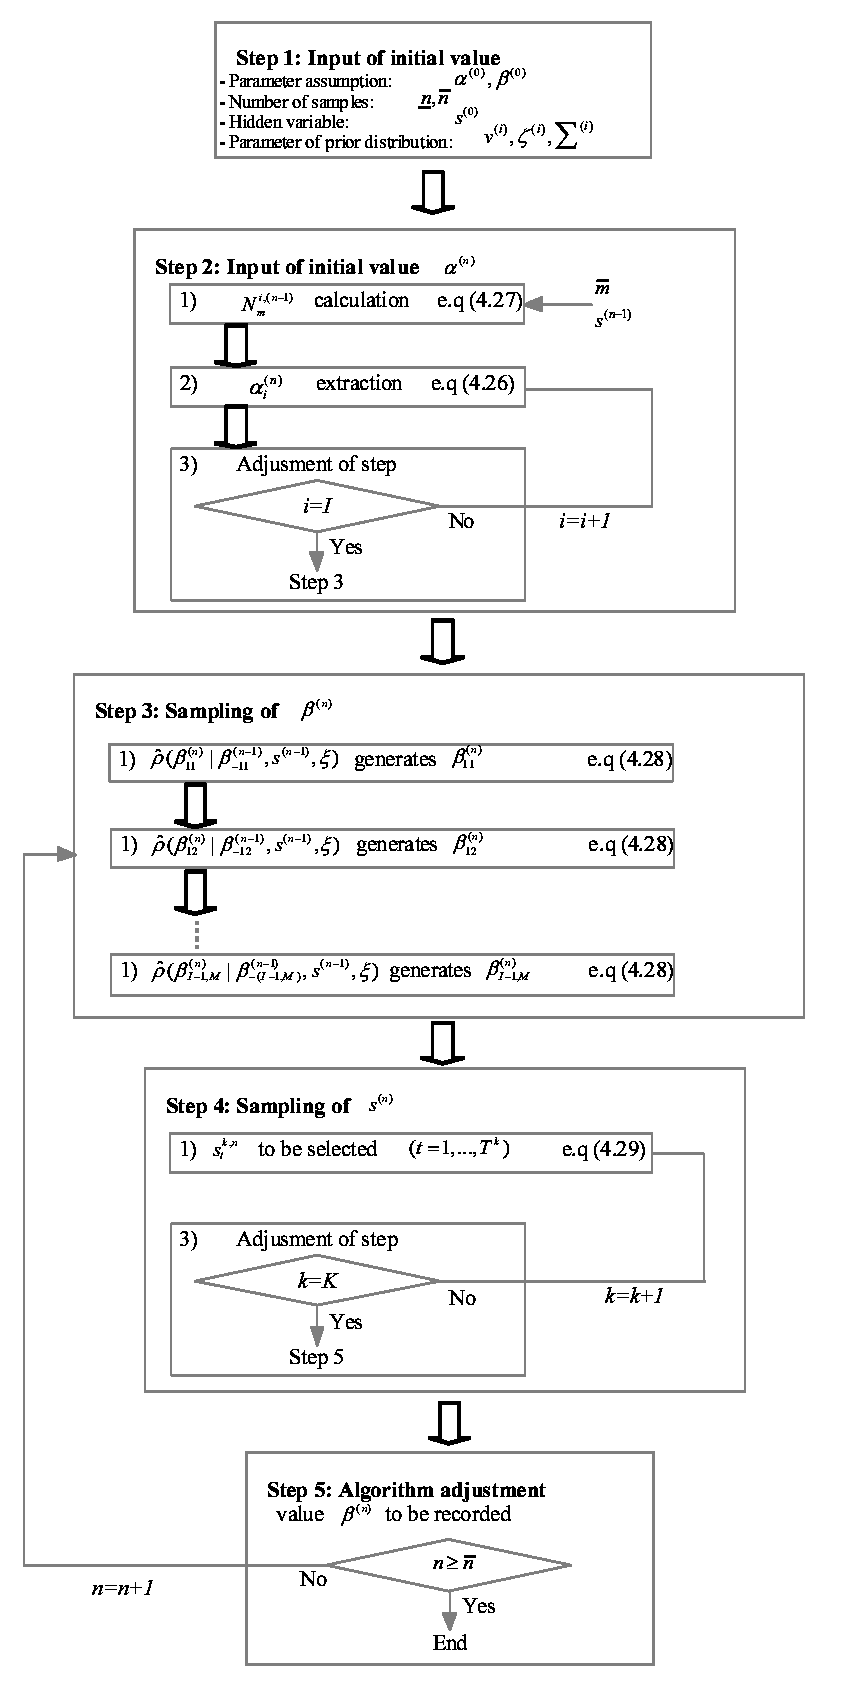
\includegraphics[scale=0.8]{fig44.eps}
\end{center}
\caption{Flowchart of Bayesian Estimation for Hidden Markov Model}
\label{fig44}
\end{footnotesize}
\end{figure}
%%%%%%%%%%%%
\subsubsection{Step 1: Initial parameter values} \label{4541}
Parameter vectors $\mbox{\boldmath$\nu$}^i~(i=1,\cdots,I)$, $\mbox{\boldmath$\zeta$}_i$, and $ \mbox{\boldmath$\Sigma$}_i~(i=1,\cdots,I-1)$ of the prior probability distribution in equations (\ref{nu11}) and (\ref{Kseiki}) have an arbitrarily set of values. The value of the hidden variable $\mbox{\boldmath$s$}^{(0)}=(\mbox{\boldmath$s$}^{(1,0)},\cdots,\mbox{\boldmath$s$}^{(K,0)})$ is initially chosen so as to satisfying $\mbox{\boldmath$s$}^{(k,0)}=(s_1^{k,0},\cdots,s_T^{k,0})$, $1\leq s_1^{k,0}\leq \cdots \leq s_T^{k,0}\leq I$, and $m_t^k\leq s_t^{k,0}~(t=1,\cdots,T;k=1,\cdots,K)$. The influence of the initial values $\mbox{\boldmath$\alpha$}^{(0)}$ and $\mbox{\boldmath$\beta$}^{(0)}$ gradually becomes weaker as more information generated by MCMC simulation is accumulated. To begin with the iteration, a sampling number $n$ in MCMC simulation is assigned as $n=1$.
%%%%%%%%%%%%%%
\subsubsection{Step 2: Sampling of the parameter $\mbox{\boldmath$\alpha$}^{(n)}$} 
\label{4542}
This section describes the estimation of $\mbox{\boldmath$\alpha$}^{(n)}=(\mbox{\boldmath$\alpha$}_1^{(n)},\cdots,\mbox{\boldmath$\alpha$}_{I-1}^{(n)})$ based on the prior hidden variable $\mbox{\boldmath$s$}^{(n-1)}$. The probability density function $\rho(\mbox{\boldmath$\alpha$}^{(n)}|\mbox{\boldmath$s$}^{(n-1)},\mbox{\boldmath$\xi$})$ in equation (\ref{k1}) can be re-written, with an extended description $\mbox{\boldmath$\alpha$}_i^{(n)}$ $=(\alpha_m^{i,n}:m=1,\cdots,i)$:
\begin{eqnarray}
&&  \tilde{\rho}(\mbox{\boldmath$\alpha$}_i^{(n)}|\mbox{\boldmath$s$}^{(n-1)},\mbox{\boldmath$\xi$}) 
 \propto \left\{ \prod_{k=1}^K \prod_{t=1}^{T^k} \alpha_{\bar{m}_t^k}^{s_{t}^{k,(n-1)}} \right\}\left\{\prod_{m=1}^{i} (\alpha_m^{i,n})^{\nu_m^{i}-1} \right\}  \nonumber \\
 && \hspace{20mm}=\prod_{m=1}^i (\alpha_m^{i,n})^{\nu_m^{i}+N_m^{i,(n-1)}-1}, \label{dir}
\end{eqnarray}
where $N_m^{i,(n-1)}$ is defined in the following equation, particularly when the values of the condition state $\bar{\mbox{\boldmath$m$}}$ and the hidden variable $\mbox{\boldmath$s$}^{(n-1)}$ are available:
\begin{eqnarray}
&& N_m^{i,(n-1)}=\#\Big\{\bar{m}_t^k=m \cap s_t^{k,(n-1)}=i\Big\}. \label{lllll}
\end{eqnarray}
The indication $\#\{\}$ in equation (\ref{lllll}) presents the number of measurable samples, to which the equation in the parentheses $\{�\}$ is referred. The parameter $\mbox{\boldmath$\alpha$}$ in equation (\ref{dir}) is assumed to follow the Dirichlet distribution, with its parameter as $\nu_m^{i}+N_m^{i,(n-1)}-1$. The parameters of the Dirichlet distribution is subsequently updated by using the extracted samples  $\mbox{\boldmath$\alpha$}_i^{(n)}=(\alpha_1^{i,(n)}, \cdots,\alpha_{i}^{i,(n)})$ through Gibbs sampling. It is noted that the samples of the parameter $\mbox{\boldmath$\alpha$}_i^{(n)}$ are evaluated from the entire range of the condition state $i(i=1,...,I)$.
%%%%%%%%%%%
\subsubsection{Step 3: Sampling of the parameter $\mbox{\boldmath$\beta$}^{(n)}$} \label{4543}
This section describes an algorithm for estimating the unknown parameter $\mbox{\boldmath$\beta$}$ of the multi-stage exponential hazard model (See the Appendix). Additional notation of the unknown parameter is $\mbox{\boldmath$\beta$}_{-eq}$. It is noticed from the notation that the element $\beta_{eq}$ $(e,q)~(e,q=1,\cdots,M)$ is excluded from the list of the unknown parameter $\mbox{\boldmath$\beta$}$. Thus, we formulated the conditional probability density function $\rho(\beta_{eq}|\mbox{\boldmath$\beta$}_{-eq},\mbox{\boldmath$s$},\mbox{\boldmath$\xi$})$ of $\beta_{eq}$ based on the assumed value of $\mbox{\boldmath$\beta$}_{-eq}$ in equation (\ref{k2}):
%
   \begin{eqnarray}
      && \hspace{-5mm} \hat{\rho}(\beta_{eq}|\mbox{\boldmath$\beta$}_{-eq},\mbox{\boldmath$s$},
      \mbox{\boldmath$\xi$}) \propto \prod_{i=1}^{e} \prod_{j=e}^I \prod_{k=1}^K  \prod_{t=1}^{T^k} \Bigl\{ \prod_{l=i}^{j-1} (\theta_l^k)^{\delta_{ij}^{tk}-\delta_{ie}^{tk}} \sum_{h=i}^{j} 
      \cdot \prod_{l=i,\neq h}^{h-1}\frac{1}{\theta_{l}^k-\theta_{h}^k} \exp (-\theta_{h}^k z_t^k)\Bigl\}^{\delta_{ij}^{tk}} \nonumber \\
      &&\hspace{50mm} \cdot \prod_{i=1}^{I-1}\exp\Big\{-\frac{1}{2}
      (\mbox{\boldmath$\beta$}_i-\mbox{\boldmath$\zeta$}_i)
      \mbox{\boldmath$\Sigma_i$}^{-1}
      (\mbox{\boldmath$\beta$}_{i}-\mbox{\boldmath$\zeta$}_i)^\prime\Big\}\Bigr] \nonumber \\
      && \hspace{2mm} \propto
\prod_{i=1}^{e} \prod_{j=e}^I \prod_{k=1}^K  \prod_{t=1}^{T^k} \Bigl[ \prod_{l=i}^{j-1} \{\exp(\beta_{eq} x_q^k)\}^{\delta_{ij}^{tk}-\delta_{ie}^{tk}}  
      \sum_{h=i}^{j} \prod_{l=i,\neq h}^{h-1}\frac{1}{\theta_{l}^k-\theta_{h}^k} \exp (-\theta_{h}^k z_t^k)\Bigl]^{\delta_{ij}^{tk}} \nonumber \\
&& \hspace{50mm} \exp\Big\{-\frac{\sigma_{e}^{qq}}{2}(\beta_{eq}-\hat{\zeta}_{e}^q)^2 \Big\}. \nonumber \\
&& \hspace{50mm}
      \hat{\zeta}_{e}^q
      = \zeta_{e}^q+\sum_{h=1,\neq q}^{M}(\beta_{eh}-\zeta_{e}^h)\sigma_e^{hq},
       \label{condition1}
      \end{eqnarray}
%
%
where $\delta_{ie}^{tk}$ and $\delta_{ij}^{tk}$ are dummy variables:
\begin{eqnarray}
&& \delta_{ie}^{tk}=\left\{
\begin{array}{ll}
1 & \hspace{2mm} \text{when} \hspace{2mm} s_{t-1}^k=i=e\\
0 &  \text{otherwise}
\end{array}
\right. 
\hspace{3mm} and \hspace{3mm} \delta_{ij}^{tk}=\left\{
\begin{array}{ll}
1 & \hspace{2mm} \text{when} \hspace{2mm} s_{t-1}^k=i,~s_t^k=j \\
0 & \text{otherwise}	
\end{array},
\right. \nonumber
\end{eqnarray}
$\zeta_{e}^q$ and $\sigma_{e}^{hq}$ are the prior expected values of the vector $\mbox{\boldmath$\zeta$}_e$ and the prior standard covariance of entire procession $\mbox{\boldmath$\Sigma_e$}^{-1}$ with respect to condition state $q$ and $(h,q)$. In addition, $\sum_{h=1,\neq q}^{M}$ is the summation of all condition states from $\sum_{h=1,\neq q}^{M}$, excluding the condition state $q$. The expected condition state is generated by using the conditional probability density functions. By using the generated condition states, we can come up with the posterior distribution of the parameter $\mbox{\boldmath$\beta$}$. A detailed MCMC simulation for estimating the posterior distribution is further presented in the subsequent writing. However, to this point, a summation of the random sampling procedure for the parameter $\mbox{\boldmath$\beta$}^{(n)}=(\beta_{11}^{(n)},\cdots,\beta_{I-1M}^{(n)})$ is presented as follows:
%%%
\begin{itemize}
\item {Step 3.1 - value of parameter $\beta_{11}^{(n)}$ is randomly generated from 
$\hat{\rho}(\beta_{11}^{(n)}|\mbox{\boldmath$\beta$}_{-11}^{(n-1)}$, $\mbox{\boldmath$s$}^{(n-1)},\mbox{\boldmath$\xi$})$}.
%%%
\item{Step 3.2 - value of parameter $\beta_{12}^{(n)}$ is randomly generated from $\hat{\rho}(\beta_{12}^{(n)}|\mbox{\boldmath$\beta$}_{-12}^{(n-1)}$, $\mbox{\boldmath$s$}^{(n-1)},\mbox{\boldmath$\xi$})$}.
%%%
\item{Step 3.3 - similar procedure in step 3.1 and step 3.2 is repeated.}
%%
\item{Step 3.4 - value of parameter $\beta_{I-1M}^{(n)}$ is randomly generated from  $\hat{\rho}(\beta_{I-1,M}^{(n)}| \\ \mbox{\boldmath$\beta$}_{-(I-1M)}^{(n-1)},  \mbox{\boldmath$s$}^{(n-1)},\mbox{\boldmath$\xi$})$.}
\end{itemize}
Gibbs sampling is applied to generate the condition states from $(I-1)M$ conditional posterior probability density functions. The so-called ``adaptive sampling rejection'' \cite{gilks} is used as a technique to generate the specimens of the parameter in the posterior distribution, which is explained in equation (\ref{condition1}).
%%%%%%%%%%%%%%
\subsubsection{Step 4: Updating the hidden variable} \label{4544}
Given the prior value of the hidden variable $\mbox{\boldmath$s$}_{-t}^{k,(n-1)}=(s_1^{k,n},\cdots,s_{t-1}^{k,n},s_{t+1}^{k,(n-1)},\cdots,s_{T^k}^{k,(n-1)})$, a new hidden variable $\mbox{\boldmath$s$}^{(n)}$ is randomly selected based on the conditional probability law in equation (\ref{k3}). Random generation applies for all condition states $s_t^{k,n} ~(s_t^{k,n} \in \{s_{t-1}^{k,n},\cdots, s_{t+1}^{k,(n-1)}\})$. Thus, we can come up with the conditional probability for the hidden variable $s_t^{k,n} ~(s_t^{k,n} \in \{s_{t-1}^{k,n},\cdots, s_{t+1}^{k,(n-1)}\})$:
%%%
\begin{eqnarray}
&& \hspace{-15mm} \mbox{Prob}\{s_t^k=i|\mbox{\boldmath$\alpha$},\mbox{\boldmath$s$}_{-t}^{k,(n-1)},\mbox{\boldmath$\xi$}\} 
 =\left\{
\begin{array}{l}
\frac{\omega_{it}^{k,(n-1)} f_i(m_t^k|\mbox{\boldmath$\alpha$}_i^{(n)})}{\sum_{j=1}^{s_{2}^{k,(n-1)}} \omega_{jt}^{k,(n-1)} f_j(m_t^k|\mbox{\boldmath$\alpha$}_j^{(n)})} \hspace{10mm} (at \hspace{5mm} t=1) \\
\frac{\omega_{it}^{k,(n-1)} f_i(m_t^k|\mbox{\boldmath$\alpha$}_i^{(n)})}{\sum_{j=s_{t-1}^{k,n}}^{s_{t+1}^{k,(n-1)}} \omega_{jt}^{k,(n-1)} f_j(m_t^k|\mbox{\boldmath$\alpha$}_j^{(n)})} \hspace{10mm} (2\leq t <T^k) \\
\frac{\omega_{it}^{k,(n-1)} f_i(m_t^k|\mbox{\boldmath$\alpha$}_i^{(n)})}{\sum_{j=s_{t-1}^{k,n}}^I \omega_{jt}^{k,(n-1)} f_j(m_t^k|\mbox{\boldmath$\alpha$}_j^{(n)})} \hspace{10mm}(at \hspace{5mm}t=T^k) 
\end{array},
\right.\label{k33}
\end{eqnarray}
where
\begin{eqnarray}
&& \omega_{jt}^{k,(n-1)}=\left\{
\begin{array}{ll}
\pi_{1j}\pi_{js_2^{k,(n-1)}} & t=1 \\
\pi_{s_{t-1}^{k,n}j}\pi_{js_{t+1}^{k,(n-1)}} & 2\leq t < T^k \\
\pi_{s_{T^k-1}^{k,n}j} & t=T^k
\end{array}.
\right.
\end{eqnarray}
The hidden variable $s_t^{k,n}~(t=1,\cdots,T^k)$ is estimated one after the other,  starting from $t=1$ for all number of the sample $k~(k=1,\cdots,K)$.
%%%%%%%%%%%%%%
\subsubsection{Step 5: Determining algorithm adjustment} \label{4545}
After step \ref{4544}, value of the parameters $\mbox{\boldmath$\alpha$}^{(n)}$, $\mbox{\boldmath$\beta$}^{(n)}$ and the hidden variable $\mbox{\boldmath$s$}^{(n)}$ are recorded. At the iteration $n=n+1$, the program returns to the step \ref{4542}. If the algorithm satisfies $n\leq \overline{n}$, the program will terminate. 

A major concern is the number of the condition state $n$ generated by the program. The number should be carefully examined. In several cases, the steady condition states could not be reached even though a large number of condition states had been accumulated. It is therefore desirable to eliminate the problem by introducing a minimum set of the parameter value as $\underline{n}$. In fact, values of the parameters $\mbox{\boldmath$\alpha$}^{(n)}$ and $\mbox{\boldmath$\beta$}^{(n)}~(n=\underline{n}+1,\underline{n}+2,\cdots,\overline{n})$ are embedded in the posterior probability density function $\rho(\mbox{\boldmath$\alpha$},\mbox{\boldmath$\beta$}|\mbox{\boldmath$\xi$})$ through the Gibbs sampling. As a result, the estimation for the posterior distribution of the parameters $\mbox{\boldmath$\alpha$},\mbox{\boldmath$\beta$}$ becomes analytical feasible. To verify the estimation results, we applied the Geweke statistical test.  
%%%% 
 \subsection{Posterior distribution statistic} \label{455}
Statistical testing for the parameter $\mbox{\boldmath$\alpha$}$ and $\mbox{\boldmath$\beta$}$ can be carried out based on the samples generated by using the MCMC simulation. However, in the simulation, the probability density function $\rho(\mbox{\boldmath$\alpha$},\mbox{\boldmath$\beta$}|\mbox{\boldmath$\xi$})$ cannot  be considered as an analytical function. Therefore, instead of using the full parametric approach for statistical testing, non-parametric approach is recommended. From the Gibbs sampling, the samples concerning $\mbox{\boldmath$\theta$}^{(n)}=(\mbox{\boldmath$\alpha$}^{(n)},\mbox{\boldmath$\beta$}^{(n)})~(n=1,\cdots,\overline{n})$ are generated. Among the generated samples, the first $\underline{n}$ samples will be removed. A new set of samples will then be defined as a replacement, with its subcriptions as ${\cal M}=\{\underline{n}+1,\cdots,\overline{n})$. By applying this approach, the joint probability distribution functions $G(\mbox{\boldmath$\alpha$})$ and $G(\mbox{\boldmath$\beta$})$ can be defined:
 %
 %
   \begin{eqnarray}
 && G(\mbox{\boldmath$\alpha$})
      =\frac{\mbox{\#}(\mbox{\boldmath$\alpha$}^{(n)}
      \leq \mbox{\boldmath$\alpha$}, n\in {\cal M})}
      {\overline{n}-\underline{n}}, \\
      && G(\mbox{\boldmath$\beta$})
      =\frac{\mbox{\#}(\mbox{\boldmath$\beta$}^{(n)}
      \leq \mbox{\boldmath$\beta$}, n\in {\cal M})}
      {\overline{n}-\underline{n}},
   \end{eqnarray}
 %
 %
where $\mbox{\#}(\mbox{\boldmath$\beta$}^{(n)} \leq \mbox{\boldmath$\beta$}, n\in {\cal M})$ is regarded as the total number of samples, from which the logical expression $\mbox{\boldmath$\beta$}^{(n)} \leq \mbox{\boldmath$\beta$}, n\in {\cal M}$ is satisfied. Moreover, the expected values of the posterior distribution of $\tilde{\mbox{\boldmath$\zeta$}_i}(\mbox{\boldmath$\beta$}_i)$ and standard covariance $\tilde{\mbox{\boldmath$\Sigma$}_i}(\mbox{\boldmath$\beta$}_i)$ are defined respectively as follows:
%
   \begin{eqnarray}
      && \hspace{-7mm}
      \tilde{\mbox{\boldmath$\zeta$}_i}(\mbox{\boldmath$\beta$}_i)=
      (\tilde{\zeta}(\beta_{i,1}),\cdots,\tilde{\zeta}
      (\beta_{i,M}))^\prime =\Big(\sum_{n=\underline{n}+1}^{\overline{n}}
      \frac{\beta_{i,1}^{(n)}}{\overline{n}-\underline{n}},
      \cdots, \sum_{n=\underline{n}+1}^{\overline{n}}
      \frac{\beta_{i,M}^{(n)}}{\overline{n}-\underline{n}}\Big)^\prime,
      \label{mu3} \\
 %
      && \hspace{-7mm}
      \tilde{\mbox{\boldmath$\Sigma$}_i}(\mbox{\boldmath$\beta$}_i)=
      \left(
      \begin{array}{lll}
         \tilde{\sigma}^2(\beta_{i,1}) & \cdots
            & \tilde{\sigma}(\beta_{i,1}\beta_{i,M}) \\
         \vdots & \ddots & \vdots \\
         \tilde{\sigma}(\beta_{i,M}\beta_{i,1}) & \cdots
            & \tilde{\sigma}^2(\beta_{i,M}) \\
      \end{array}
      \right),
      \label{mu4}
   \end{eqnarray}
 %
 %
where
%
 %
   \begin{eqnarray}
      && \hspace{-3mm} \tilde{\sigma}^2(\beta_{i,m})=
      \sum_{n=\underline{n}+1}^{\overline{n}}
      \frac{\{\beta_{i,m}^{(n)}-\tilde{\zeta}(\beta_{i,m})\}^2}
      {\overline{n}-\underline{n}}, \\
      && \hspace{-3mm} \tilde{\sigma}(\beta_{i,m}\beta_{i,l}) 
       =\sum_{n=\underline{n}+1}^{\overline{n}}
      \frac{\{\beta_{i,m}^{(n)}-\tilde{\zeta}(\beta_{i,m})\}
      \{\beta_{i,l}^{(n)}-\tilde{\zeta}(\beta_{i,l})\}}{\overline{n}-\underline{n}}.
      \nonumber 
    \end{eqnarray}
 %
 %
The confidence interval of the parameter $\mbox{\boldmath$\alpha$}$ and $\mbox{\boldmath$\beta$}$ are examined and determined by using the samples generated from Gibbs sampling. For example, the $100(1-2\varepsilon)\%$ confidence interval of the parameter $\mbox{\boldmath$\beta$}$ is defined by using statistical sampling order  $(\underline{\beta}^{\varepsilon}_{i,m},\overline{\beta}^{\varepsilon}_{i,m})~(i=1,\cdots,I-1,\quad m=1,\cdots,M)$ with $\underline{\beta}^{\varepsilon}_{i,m}< \beta_{i,m} <\overline{\beta}^{\varepsilon}_{i,m}$:
%%%
 \begin{eqnarray}
      && \hspace{-8mm} \underline{\beta}^{\varepsilon}_{i,m}
      =\arg \max_{\beta_{i,m}^\ast} 
       \left\{ \frac{\#(\beta_{i,m}^{(n)} \leq \beta_{i,m}^\ast,n
      \in {\cal M})}
      {\overline{n}-\underline{n}}\leq \varepsilon \right\}, \label{sin1} \\
 %
      && \hspace{-8mm} \overline{\beta}^{\varepsilon}_{i,m}
      =\arg \min_{\beta_{i,m}^{\ast\ast}} 
      \left\{ \frac{\#(\beta_{i,m}^{(n)} \geq
      \beta_{i,m}^{\ast\ast},n\in {\cal M})}
      {\overline{n}-\underline{n}}\leq \varepsilon \right\}. \label{sin2}
   \end{eqnarray}
 %
 %
It is noted that the initial value of the parameter $\mbox{\boldmath$\theta$}^{(0)}$ does not guarantee to have the true condition states neither for prior distribution and posterior distribution in MCMC simulation. Thus, it is necessary to consider $\overline{n}$ samples generated by Gibbs sampling as the posterior distribution of the first $\underline{n}$ set $\mbox{\boldmath$\theta$}^{(n)}=(\mbox{\boldmath$\alpha$}^{(n)},\mbox{\boldmath$\beta$}^{(n)})~(n=1,\cdots,\underline{n})$. When the number of samples increases to be $\underline{n}+1$, a hypothetical test using the Geweke statistical test is performed to verify whether the samples coming from the prior or the posterior distribution \cite{geweke}. In the next step, the sampling distribution $\mbox{\boldmath$\theta$}^{(n)}~(n=1,\cdots,\overline{n})$ is divided into two subsets $n_1$ and $n_2$. In the Geweke statistical test, the ranges of the two subsets are recommended as $n_1=0.1(\overline{n}-underkine{n})$ and $n_2=0.5(\overline{n}-underkine{n})$ respectively \cite{geweke}. According to \citet{chib1,newe1}, the Geweke statistical test used to verify the value of the parameter $\alpha$ can be outlined as follows:
\begin{eqnarray}
&& Z_{\alpha_m^i}=\frac{{}_1\bar{\alpha}_m^i-{}_2\bar{\alpha}_m^i}{\sqrt{\nu_1^2(\alpha_m^i)+\nu_2^2(\alpha_m^i)}}\sim  {\cal N}(0,1),\label{loo} \\
&& {}_1\bar{\alpha}_m^i = \frac{\sum_{k=\underline{n}+1}^{\underline{n}+n_1} \alpha_m^{i,k}}{n_1}, \quad {}_2\bar{\alpha}_m^i=\frac{\sum_{k=\overline{n}-n_2+1}^{\overline{n}} \alpha_m^{i,k}}{n_2}, \quad \nonumber \\ 
&&
 \nu_1^2(\alpha_m^i)=\frac{2\pi \hat{f}_{\alpha_m^i}^1(0)}{n_1}, \quad \nu_2^2(\alpha_m^i)=\frac{2\pi \hat{f}_{\alpha_m^i}^2(0)}{n_2}, \nonumber
\end{eqnarray}
where ${f} _ {\alpha_m^i} ^l(x) ~ (l=1,2) $ is the probability density function and the value of $2\pi{f} _ {\alpha_m^i} ^l(0) $ is estimated from the following equations:
\begin{eqnarray}
&& 2\pi \hat{f}_{\alpha_m^i}^l(0)={}_l\hat{\omega}_0+2\sum_{s=1}^q w(s,q){}_l\hat{\omega}_m^i,  \\
&& {}_1\hat{\omega}_0=n_1^{-1}\sum_{g=\underline{n}+1}^{\underline{n}+n_1}(\alpha_m^{i,g}-{}_1\bar{\alpha}_m^i)^2, \quad
{}_2\hat{\omega}_0=n_2^{-1}\sum_{g=\overline{n}-n_2+1}^{\overline{n}}(\alpha_m^{i,g}-{}_2\bar{\alpha}_m^i)^2,\nonumber \\
&& {}_1\hat{\omega}_m^i=n_1^{-1}\sum_{g=\underline{n}+s+1}^{\underline{n}+n_1}(\alpha_m^{i,g}-{}_1\bar{\alpha}_m^i)(\alpha_m^{i,(g-s)}-{}_1\bar{\alpha}_m^i), \quad \nonumber \\
&&{}_2\hat{\omega}_m^i=n_2^{-1}\sum_{g=\overline{n}-n_2+s+1}^{\overline{n}}(\alpha_m^{i,g}-{}_2\bar{\alpha}_m^i)(\alpha_m^{i,(g-s)}-{}_2\bar{\alpha}_m^i), \nonumber \\
&& w(s,q)=1-\frac{s}{q+1}. \nonumber
\end{eqnarray}
The value of coefficient $q$, which represents for the approximate value of the spectrum density, should equals to $20$ as recommended in the practice of the Geweke statistical test \cite{geweke}. In a similar approach, a statistical testing for the parameter $\beta_{i,m}~(i,m=1,\cdots,M)$ using the Geweke statistical test can also be performed:
\begin{eqnarray}
&& Z_{\beta_{i,m}}=\frac{{}_1\bar{\beta}_{i,m}-{}_2\bar{\beta}_{i,m}}{\sqrt{\nu_1^2(\beta_{i,m})+\nu_2^2(\beta_{i,m})}}\sim{\cal N}(0,1),\label{looo} \\
&& {}_1\bar{\beta}_{i,m}=\frac{\sum_{k=\underline{n}+1}^{\underline{n}+n_1} \beta_{i,m}^{(k)}}{n_1}, \quad {}_2\bar{\beta}_{i,m}=\frac{\sum_{k=\overline{n}-n_2+1}^{\overline{n}} \beta_{i,m}^{(k)}}{n_2} , \quad \nonumber \\
&& \nu_1^2(\beta_{i,m})=\frac{2\pi \hat{f}_{\beta_{i,m}}^1(0)}{n_1}, \quad \nu_2^2(\beta_{i,m})=\frac{2\pi \hat{f}_{\beta_{i,m}}^2(0)}{n_2}. \nonumber
\end{eqnarray}
In this test, the null hypothesis $H_0$ and the alternative hypothesis $\alpha_m^i$ concerning the invariance distribution of the setting-values for the parameter $\alpha_m^i$ can be defined as
\begin{eqnarray}
&& \left\{
\begin{array}{ll}
H_0: |Z_{\alpha_m^i}|\leq z_{\psi/2} \\
H_1: |Z_{\alpha_m^i}|>z_{\psi/2}
\end{array},
\right.
\end{eqnarray}
where $z_{\psi/2}$ is the critical value to be applied for rejecting the null hypothesis. If the given hypothesis is accepted, the null hypothesis can be defined by a significant level $\psi\%$, to which the condition $z_{\psi/2}$ $\psi/2\%=1-\Phi(z_{\psi/2})$ is satisfied. $\Phi(z)$ is the distribution function of the standard normal distribution. As for the hypothetical testing for the distribution of the parameter $\beta_{i,m}~(i,m=1,\cdots,M)$, a similar approach can be applied.
%%%%%%%%%%%%
\section{Empirical application} \label{46}
\subsection{Overview} \label{461}
In the empirical analysis, we present the applicability of the hidden Markov model to estimate the Markov transition probabilities. In addition, we compare the obtained estimation results with the Markov transition probabilities obtained by using the multi-state exponential Markov model on the same source of the monitoring data. We use the monitoring data of the National road system of Japan. The monitoring data consists of values of various structural and performance indexes such as Elastic modulus, Thickness of pavement structures, Roughness, Flatness, Cracking, Rut, Annual traffic volume, etc. The monitoring data has been collected since the year 1986, when the advanced monitoring and inspection technologies were introduced, using high-speed inspection cars. After a rigorous verification of the monitoring data, we select the monitoring data in the period from 1998 to 2005. The total number of road sections are $5,261$, with $100$ meters for average length of each section.

In order to define the most appropriate discrete numbers of the condition states, we apply sensitivity analysis. The sensitivity analysis is substantial to verify the range of the condition states. Because, the condition states can be assumed in various discrete domains based on the actual values of performance indexes. In fact, the values of performance indexes are measured and recorded in a small scale of their units. Based on the results of the sensitivity analysis, It is found that that the arrival times to the worst condition state are almost identical regardless of the differences in the ranges of the conditions states. Thus, for the best interest of the numerical computation, we select the range of the conditions states from $1$ to $5$, with its description given in the table \ref{table41}. Moreover, to illustrate measurement errors, which might exist in the database, we summary the numbers of samples in the table \ref{table42}. The numbers in the rows of the table reflects the numbers of condition state $i$ observed at the first inspection time (referred as pre-condition state). While, the numbers in the columns represents the numbers of condition state $j$ observed at the second inspection time (referred as post-condition state). If there is no $M\&R$ action in the inspection interval, the actual value of condition state $j$ should be always greater than that of  condition state $i$. However, as can be seen from the table, the numbers of the post-condition states with better condition state than the pre-condition states have been recorded, especially with  condition state $1$ and $2$. Thus, it is implied that the monitoring data includs measurement errors.

\begin{table}
\caption{Description of Condition States.}
\label{table41}
{\small
\begin{center}
\begin{tabular}{c|c}\hline
Condition states & Range of rut values \\\hline
1 & $<$  5 mm  \\
2 & 5 mm $<$ () $<$ 10 mm \\
3 & 10mm $<$ () $<$ 15 mm \\
4 & 15mm $<$ () $<$ 20 mm \\
5 & $>$ 20 mm  \\\hline
\end{tabular}
\end{center}
}
\end{table}
%%%%
\begin{table}
\caption{Number of Samples.}
\label{table42}
\begin{center}
{\small
\begin{tabular}{c|ccccc}\hline
Pre-&\multicolumn{5}{|c}{Post-condition state}\\
Condition states & 1 & 2 & 3 & 4 & 5 \\\hline
1 &331 &339 &32 &5 &0 \\
2 &573 &1919 &468 &187 &47 \\
3 &66 & 240&382 &163 &44\\
4 & 50& 63&52 &82 &67 \\
5 & 2& 22&16 &27 &84 \\\hline
\end{tabular}
}
\end{center}
\end{table}
%%%%%%%%%%
\subsection{Estimation results} \label{462}
In the empirical study, the annual traffic volume of large-size car is considered as a main characteristic variable, which effected the deterioration or the hazard rate in equation (\ref{hazard1}). Other characteristic variables such as structural thickness is excluded since the thickness of road sections are uniform in the national construction and design standard. Denotation for the maximum traffic volume is $x_{i2}$, which is observable. Whilst, the first characteristic variable $x_{i1}$ equals to $1$ as a constant value.

The estimation results from applying the hidden Markov model with MCMC simulation are displayed in table \ref{table43}. It is highlighted from the table that the traffic volume exerts its strong influence on the deterioration, especially for the first two condition states. The values appeared in the blankets show the lower bound and upper bound of the confidence interval corresponding to $95\%$ of significant level estimated from equations (\ref{sin1}) and (\ref{sin2}). Because of having non-negative values in the blankets, value of the parameter cannot equal to $0$ with respect to $95\%$ confident level. In addition, the values of Geweke statistical test for the unknown parameter are also presented in the last line of each row in table \ref{table43}. In the Geweke statistical test, to begin with, $2000$ samples are selected and then replaced by $10,000$ generated samples. The values of Geweke statistical test for the unknown parameter are below $1.96$ as shown in table \ref{table43}. Hence, there is a high possibility that the hypothesis ``the parameter sampling process by MCMC simulation converges to stationary state'' cannot be dismissed by $5\%$ of the significant interval.

\begin{table}
\caption{Estimation Results of Hidden Markov Model.}
\label{table43}
\begin{center}
\vspace{-3mm}
{\small
\begin{tabular}{c|cc}\hline
Condition states & Constant term&Traffic Volume (TV)\\
 & $\beta_{i1}$ & $\beta_{i2}$\\ \hline
1 & 0.280  &  0.415  \\
& (0.267,0.292) &  (0.352,0.477) \\
& 1.915 & 1.154 \\\hline
2 & 0.033 &  0.188  \\
& (0.029,0.035) &  (0.172,0.206) \\
& 0.543 & 1.128 \\\hline
3 & 0.108  &  - \\
& (0.100,0.117) & - \\
& 1.199 & - \\\hline
4 & 0.112 &  - \\
& (0.101,0.121) &-\\
& 0.753 & - \\\hline
\end{tabular}
}
\end{center}
Note) The values in the blankets show lower and upper bound values of $95\%$ confident interval. The third values in each row are obtained from Geweke statistical test.
\end{table}
%%%
Fig. \ref{figure45} demonstrates the estimation results for measurement errors concerning parameter $\alpha$. It presents the probability distribution of the function $f_i(m|\mbox{\boldmath$\alpha$}_{i})$, which reflects the variation between the observed condition states and the true condition states. Two important conclusions can be drawn from the figure: 1) when the condition state is $i=1$, measurement errors occur in small scale, 2) when the condition states are $4$ and $5$, measurement errors occur in large scale, deeming a high risk in management.

%%
\begin{figure}
\begin{footnotesize}\begin{center}
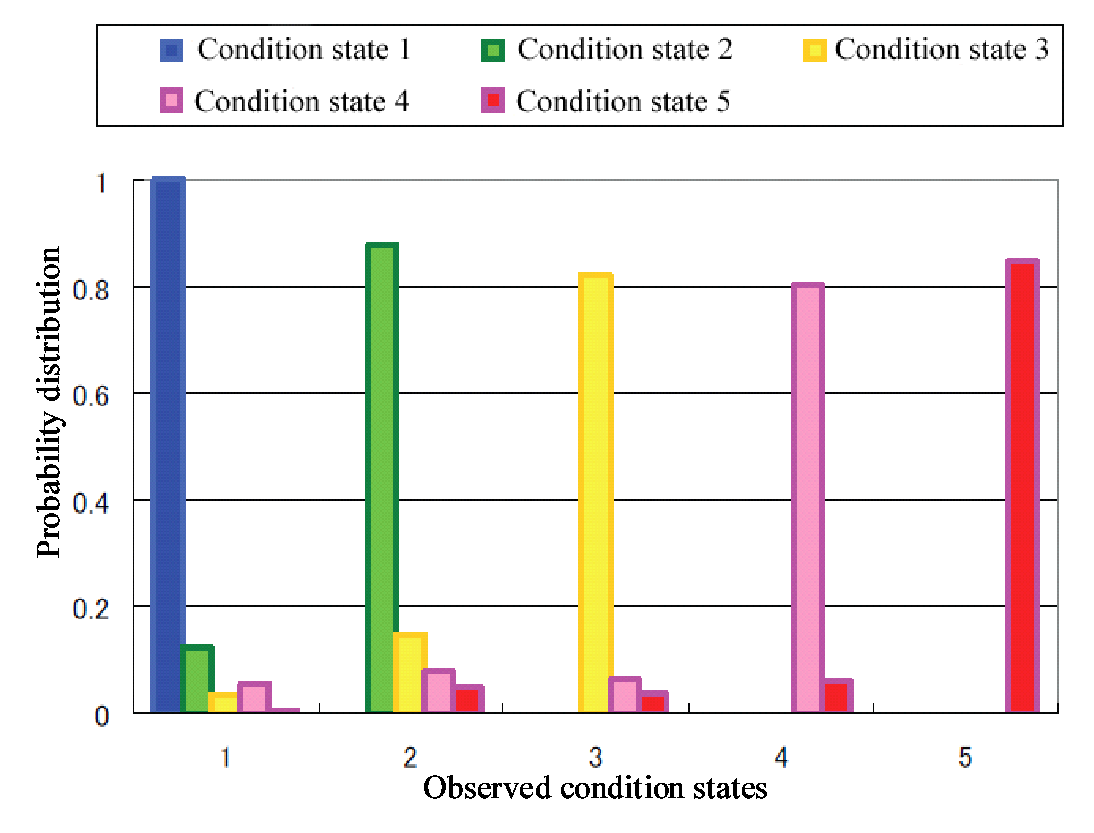
\includegraphics[scale=0.5]{fig45.eps}
\caption{Distribution of Condition State.}
\label{figure45}
\end{center}\end{footnotesize}
\end{figure}
%%%
Based on equations (\ref{hazard1}) and (\ref{17}), the values of the hazard rate and the life expectancy of condition state $i$ can be estimated. The results of estimation are presented in table \ref{table44}. It is highlighted from the table that the life expectancy of condition state $i=1$ is less than $3$ years before entering condition state $i=2$. The average life expectancy of other condition states are from $10$ to $15$ years.
%
\begin{table}
\caption{Life Expectancy of Condition States.}
\label{table44}
\begin{center}
   \vspace{-3mm}
{\small
\begin{tabular}{c|cc}\hline
   Condition states& ~$E[\theta_{il}]$~& $E[RMD_{il}^k]$(year) \\\hline
   1 & ~0.362~ & ~2.762  \\
   2 & ~0.070~ & ~14.286  \\
   3 & ~0.107~ & ~9.346 \\
   4 & ~0.112~ & ~8.929 \\
   \hline
\end{tabular}
}
\end{center}
Note) The values of the hazard rate and the life expectancy are not defined for the absorbing condition state ($i=5$) in the Markov chain model.
\end{table}
%%%%%%%%%%%%%%%%%%%%%
%\subsection{Examining analytical results} \label{sec63}
Table \ref{table45} presents the Markov transition probability matrix, which is estimated by using the hidden Markov model. The properties of the matrix are estimated based on the average hazard rates, which represent the deterioration process of the entire road sections. To compare the impact of traffic volume (TV) on the deterioration process, we categorize the traffic volume into 3 cases and estimated the hazard rates for respective cases. The benchmark case (BM case) refers to a case with use of annual average traffic volume. Whilst, another two cases considered the minimum traffic volumes and maximum traffic volumes respectively. Comparative results of three cases are presented in Figure \ref{fig46}.
%
\begin{table}
\caption{Markov transition probability - by hidden Markov model.}
\label{table45}
\begin{center}
{\small
\begin{tabular}{c|ccccc}\hline
Condition&\multicolumn{5}{|c}{Condition states}\\
States & 1 & 2 & 3 & 4& 5 \\\hline
1 & 0.696  & 0.293 & 0.011 & 0.000& 0.000 \\
2 & 0.0  & 0.932 & 0.064 & 0.003& 0.000 \\
3 & 0.0  & 0.0 & 0.898 & 0.096& 0.006 \\
4 & 0.0  & 0.0 & 0.0 & 0.894& 0.106 \\
5 & 0.0  & 0.0 & 0.0 & 0.0& 1.0 \\\hline
\end{tabular}
}
\end{center}
Note) Interval of transition is one year. 
\end{table}
%
\begin{figure}
\begin{footnotesize}
\begin{center}
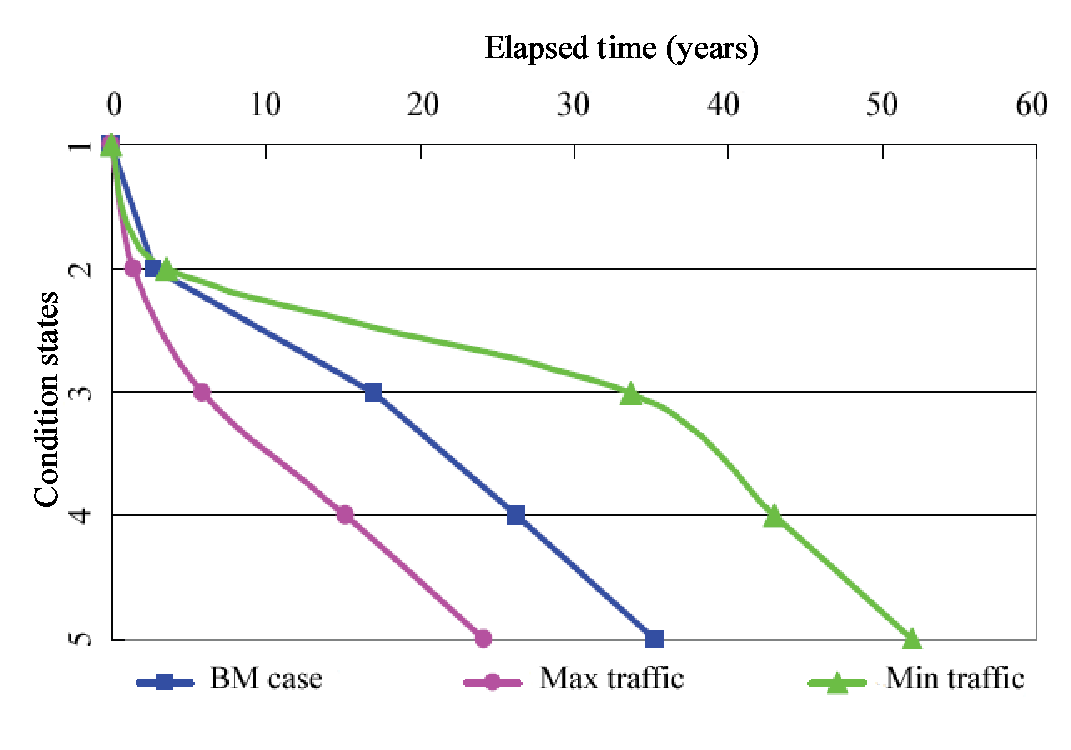
\includegraphics[scale=0.5]{fig46.eps}
\caption{Deterioration curves - traffic volume comparision.}
\label{fig46}
\end{center}
\end{footnotesize}
\end{figure}
%

An appealing conclusion from Fig.\ref{fig46} is that the traffic volume has a high impact on the deterioration process of the road. A sharp decrease in the deterioration curve is observed with the case of maximum traffic volume. In addition, there happen a long delay of the transition from  condition state $2$ to condition state $3$ for all three cases. The deterioration curve of the maximum traffic volume case shows a short life expectancy of condition state $2$. In contrary, the life expectancy of condition state $2$ of the minimum traffic volume case is about $30$ years. The life expectancies of condition state $3$ and $4$ have a similar duration.
%%%%%%%%%%%
\subsection{Measurement errors and estimation bias} \label{463}
To understand the effects of measurement errors on the estimation results, we further examine the estimation of the hidden Markov hazard model on three different databases extracted from the same source of the monitoring data, which is also used in the estimation of the exponential Markov hazard model. The first database (or filtered DB) does not include the samples, which are represented by the dots under the $45^o$ line in figure \ref{fig41}. The second database (corrected DB) is selected based on the first database, with correction of all condition states in the second inspection time appeared to have their values better than that of the first inspection time. The condition states are assumed equal to the condition states of the first inspection time. The third database (reproduced DB) is generated database by using the MCMC simulation, with use of the estimation results in the table \ref{table43}.

A comparative estimation result of the three cases is presented in table \ref{table46}. The values of the parameters under the filtered DB and corrected DB cases are obtained by using the exponential Markov hazard model, whilst, the hidden Markov model is used for estimation with the reproduced DB. The average hazard rates $E[\theta_{il}]$ of three cases are shown in table \ref{table47}.
%%%%

\begin{table*}[t]
\caption{Estimation results for unknown parameters.}
\label{table46}
\begin{center}
\vspace{-3mm}
{\scriptsize
\begin{tabular}{c|cc|cc|cc}\hline
& \multicolumn{2}{|c|}{Filtered DB} & \multicolumn{2}{|c}{Corrected DB}& \multicolumn{2}{|c}{Reproduced DB} \\\cline{2-7}
Condition & Constant term&TV & Constant term&TV& Constant term&TV \\\cline{2-7}
 states & $\beta_{i1}$ & $\beta_{i2}$ & $\beta_{i1}$ & $\beta_{i2}$ & $\beta_{i1}$ & $\beta_{i2}$  \\ \hline
 & 0.247  &  0.325 & 0.214 & 0.362 & 0.270 & 0.415 \\ 
1  & (0.238,0.256) & (0.267,0.378)& (0.205, 0.224) & (0.313,0.421) & (0.257,0.288) &  (0.353,0.477) \\
  & 1.949 & 1.646 & 1.538 & 0.060 & 1.949 & 1.646 \\\hline
 & 0.046 &  0.164 & 0.037 & 0.191 & 0.034 & 0.186\\
2  & (0.043,0.047) & (0.148,0.178)& (0.033,0.038) & (0.173,0.215)& (0.030,0.036) &  (0.170,0.202) \\
  & 1.435 & 1.903 & 1.864 & 0.584 & 1.435 & 1.903 \\\hline
 & 0.139  &  - & 0.127 & - & 0.105 & - \\
3  & (0.131,0.148) & - & (0.120,0.134) & - & (0.099,0.114) &  - \\
  & 0.232 & - & 0.020 & - & 0.232 & - \\\hline
 & 0.163 &  - & 0.131 & - & 0.113 & - \\
4  & (0.150,0.183) & - & (0.118,0.143) & - & (0.101,0.121) &  - \\
  & 0.409 & - & 0.117 & - & 0.409 & - \\\hline
\end{tabular}
}
\end{center}
Note) The values in the blankets show lower and upper bound values of $95\%$ confident interval. The third value in each row is referred to value from Geweke statistical test.
\end{table*}
%%%

A comparison between estimation results of table \ref{table44} and table \ref{table47} revealed that the average hazard rate of the condition state $1$ in the case of using exponential Markov hazard model is lower than that in the case of using the hidden Markov hazard model. On the other hand, the average hazard rates of the condition state $3$ and $4$ are higher in the case of using the exponential Markov hazard model. This findings lead to a conclusion that the over-evaluation on the hazard rates of the condition states $3$ and $4$ are happened in the case of using the filtered DB and the corrected DB. Additional evidence can be realized from looking at the tails of the deterioration curves in the Fig. \ref{fig47}.

%
\begin{table}
\caption{Estimation results for average hazard rates.}
\label{table47}
\begin{center}
{\small
\begin{tabular}{c|ccc}\hline
Condition & Filtered & Corrected & Reproduced\\
States & DB & DB & DB\\\hline
1   &  0.311 & 0.286  & 0.360 \\
2 &  0.079 & 0.075 & 0.069 \\
3   & 0.139 & 0.127 & 0.107\\
4  & 0.163 & 0.131 & 0.112\\\hline
\end{tabular}
}
\end{center}
%Note) Detailed explanation is referred in section \ref{464}
\end{table}
%
%
\begin{figure}
\begin{footnotesize}
\begin{center}
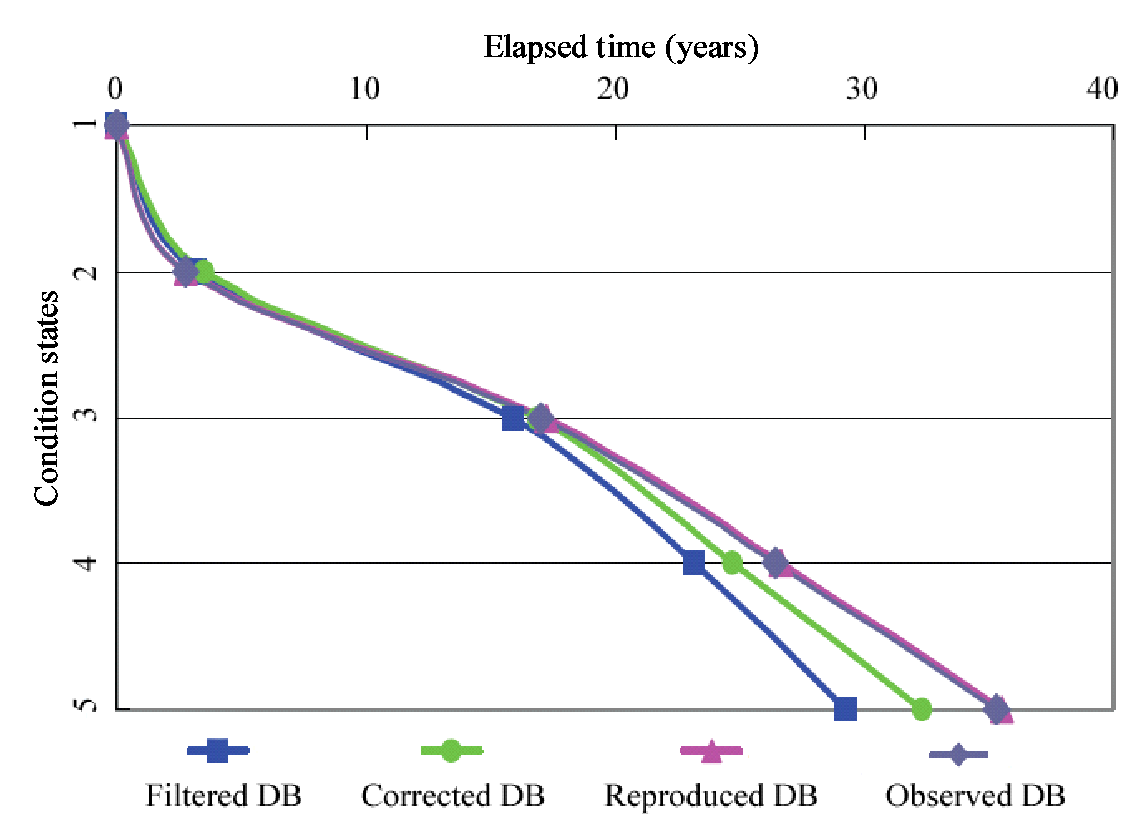
\includegraphics[scale=0.5]{fig47.eps} 
\end{center}
\end{footnotesize}
\caption{Deterioration curves - database comparision.}
\label{fig47}
\end{figure}

The problem of over-estimation on the hazard rates of condition states $i=3,4$ is because of measurement errors. Especially, in the case that $M\&R$ actions had already implemented on a number of the road sections in the past. For example, when the condition state of a road section reachs to $i=3$, mistakes in recording might happen since the corresponding values of rut index are progressing in a negligible manner. This finding suggests future study to develop a methodology to capture the transition pattern of performance indexes like the rut index in an accurate way.
%%%%%%%
\subsection{Simulation of the reproduced database} \label{464}
It is difficult to verify the accuracy of estimation results using the hidden Markov hazard model just with the observed monitoring data alone. To verify the accuracy of the estimation results, it is better to use the obtained estimation results of exponential Markov hazard model to generate the samples through the MCMC simulation. This section details the steps of simulation with the reproduced DB.

The values of parameters presented in the table \ref{table46} under the filtered DB and the corrected DB are used as the inputs of the hidden Markov hazard model. In addition, the traffic volume of large-size car is considered as a main characteristic variable. Moreover, the properties of the Markov transition probability matrix obtained by using the hidden Markov hazard model are used to update the properties of the Markov transition matrix in the exponential Markov hazard model. With this approach, the Markov transition probability $\pi_{ij}(z)$ can be repeatedly updated through equation  and (\ref{4poi}). The so-called ``virtual condition state'' at time $\tau_t^k~(t=1,\cdots,T)$ is randomly generated by using the MCMC simulation in following manners:

%%%%%%%%%%
\begin{itemize}
\item {Firstly, the observed transition probability $\pi_{1j}(z_1^k)$ at time $\tau_1^k$ is considered, with $z_1^k$ as the inspection interval counted from $t=1$. Next, the true condition state $\hat{h}(\tau_1^k)=\hat{i}$ at $\tau_i^k$ is randomly generated}.
\item {Secondly, the transition probability $\pi_{\hat{i}j}(z_2^k)$ is considered. The true condition state in this step alters to be $\hat{h}(\tau_1^k)=\hat{i}$. Next, the true condition state $\hat{h}(\tau_2^k)=\hat{j}$ is randomly generated}.
\item {Finally, the true condition state $\hat{m}(\tau_t^k)$ is randomly generated in a similar algorithm}.
\end{itemize}
%%%%%%%%%%%%%%%%
The distribution of measurement errors (as referred to Fig. \ref{figure45}) and the observed condition states $\hat{m}(\tau_t^k)$ at respective inspection times are considered in the MCMC simulation for generating sampling population. The sampling population is therefore referred as the reproduced database (reproduced DB), and used to estimate the true condition state $\hat{h}(\tau_t^k)~(t=1,\cdots,T)$. Table \ref{table46}, table \ref{table47}, and Fig. \ref{fig47} highlight that the hidden Markov hazard model has produced a better estimation result than that of using the exponential Markov model under the existence of measurement errors.
\section{Conclusion} \label{47}
In this Chapter, we have proposed an innovative analytical approach to forecast the deterioration process of infrastructure through a hidden Markov hazard model. In the model, measurement errors are considered as random variables. Measurement errors are eliminated through the assumption of prior and posterior distribution in Bayesian estimation. Furthermore, Markov Chain Monte Carlo simulation is introduced to generate random sampling population in Bayesian estimation algorithm.

We have presented an empirical study on the Japanese national road system. Estimation results reveal a fact that measurement errors have actually existed in the monitoring data, particularly concerning  condition state $3$ and $4$. Based on the estimation results of using the exponential Markov hazard model, we generate a reproduced database and use it in the hidden Markov hazard model. The estimation results are improved in the case of using the reproduced DB. 

However, we have not discussed several points, which will be considered as topics for extending this study in the future:
%
\begin{itemize}
\item{The empirical study is carried out only on the pavement system. However, this model can be applied for various types of infrastructure. Depending on structural characteristics and the prior knowledge of each infrastructure system, measurement errors can be considered not only as a random variable but also as in the form of a linear function}.
%
\item {The model can be extended if the hazard rate is considered in the form of mixture model. The mixture model can be useful to eliminate the effects of various factors on measurement errors}.
%
\item {Since the estimation results revealed a high risk of having measurement errors with condition state $3$ and $4$ in monitoring and inspection of pavement system, it is suggested that future research should pay attention on finding the reasons causing measurement errors on condition state $3$ and $4$}.
\end{itemize}